\chapter{Driver commande des moteurs}

\section{Introduction}

Un driver est un programme développé avec un langage reconnu pour sa proximité avec le matériel, le langage C. Et c'est la raison d'être des drivers. Ces derniers font la passerelle entre les applications qui se trouvent dans la partie utilisateur (user-space) et le matériel.

\vspace{1cm}

Le plus simple des exemples est celui du clavier. Lorsque j'appuie sur une touche pour écrire ce rapport un contact électrique est émit et informe le micro-processeur qu'une touche à été appuyée. Puis un programme, le driver du clavier, viens contrôler les entrées pour savoir quelle touche a été pressé. Et envoie cette information au système d'exploitation pour que la lettre soit affichée.

\vspace{1cm}

Le driver moteur a pour mission de permettre de contrôler les moteurs d'azimut, d'élévation et de zoom du télescope. D'informer le logiciel principal de l'accomplissement d'une manœuvre, théoriquement (explication chapitre 13.2). Il assure la sécurité du système de pilotage à bas niveau. Le système de sécurité consiste à interrompre le mouvement d'élévation ou de zoom si ils atteignent leur fin de course, le mouvement d'azimut n'étant pas soumis à cette contrainte.

\section{Fonctionnalités du driver}

\begin{figure}[H]
    \centering
    \includegraphics[width=1\linewidth]{\figures/sch_a4988_mod.png}
    \decoRule
    \caption[
    Schéma des entrées / sorties du driver moteur]{
    Schéma des entrées / sorties du driver moteur}
    \label{fig:Schéma des entrées / sorties du driver moteur}
    \end{figure}

\vspace{1cm}

La figure ci-dessus représente le driver contrôlant les moteurs. À gauche du bloc il y a les entrées et les sorties du driver d'un point de vue informatique.

\vspace{1cm}

Les entrées regroupent l'ensemble des données qu'attend le driver pour entreprendre une action, nous retrouvons de ce fait, le choix de l'action à réaliser, le nombre de pas à parcourir, et le sens de rotation et le choix du moteur. Les choix des actions à faire sont en gras à l'intérieur du bloc Driver. Comme vous pouvez le voir toutes les actions n'ont pas besoin de toutes les informations demandées en entré (comme l'action \codeinline{text}{stopOne}), dans ces cas seules les entrées nécessaires seront prises en comptes.

\vspace{1cm}

Concernant les sorties informatiques, il y a l'acquittement de réception qui a pour but de rassurer l'application en lui indiquant ce qu'il a reçu, ainsi l'application peut vérifier que les données envoyées sont correctes. Si il y a une erreur de communication l'application demande l'arrêt des moteurs et renvoi l'ordre ajusté (en prenant en compte le déplacement qui à été effectué dans l'erreur).

%\vspace{1cm}

Nous trouvons ensuite l'achèvement d'action, lorsque une action arrive a son terme (mouvement d'azimut, d'élévation, etc.), le driver l'indique à l'application, ainsi si jamais il y a un ajustement à effectuer elle renverra un ordre pour bien être placé. Et pour finir ce coté informatique, il y a le retour de code d'erreur qui survient lorsqu'un incident arrive dans le driver (ressource inaccessible (pin, timer, interruption, problème de fermeture driver ou d'ouverture, etc.).

\vspace{1cm}

Sur le dessus du driver nous trouvons 5 entrées (matérielles) capteurs. Chacun d'eux prévient de l'arrivée en butée d'un axe, excepté pour le capteur rotation azimutale qui indique juste la position du télescope en rotation lorsqu'il est activé.

Ce capteur a deux rôles, durant la phase de développement il nous permettra de déterminer le nombre exact et réel du pas pour un tour complet du télescope (ce qui permettra de développer l'algorithme de positionnement du télescope dans l'application principale). Le second rôle, plus tard, sera de faire du recalibrage de la centrale inertielle en cas de décalage entre les résultats de ce capteur et ceux de la centrale inertielle.

\vspace{1cm}

Au final à droite du bloc nous trouvons les sorties (matérielles) du driver. Ces dernières répètent le même chose pour chacun des 3 moteurs~: une pin pour le front montant pour lancer un pas moteur, le sens de rotation (0 ou 1), et 3 pins pour le choix du mode pas de rotation du moteur (pas complet, demi-pas, quart de pas, etc.).

\vspace{1cm}
  
Deux exemples de fonctionnement du driver avec ces entrées/sorties~:
\begin{itemize}[label=$\bullet$]
	\item Faire tourner le zoom de 50 pas dans le sens horaire~:
	\begin{enumerate}
		\item Réception des nombres de l'application [ 3 ; 50 ; 0 ] pour choisir la fonction zoom, nombre de pas, sens de rotation horaire.
		\item Envoi de l'accusé de réception, à l'application, contenant les nombres [ 3 ; 50 ; 0 ].
		\item Exécution de la fonction zoom avec les données [ 3 ; 50 ; 0 ] en argument.
		\item Écrit dans la sorte du moteur zoom sens de rotation: 0.
		\item Écrit en sortie de mode de pas du moteur zoom la configuration pour faire des pas complet. 
		\item Créer un timer qui va permettre de créer un front montant, tant que l'on n'a pas atteint le nombre de pas à parcourir.
		\item Si l'on a parcouru tous les pas complet et qu'il faut réaliser des pas plus fins, pour atteindre au plus près l'angle demandé, on change le mode de pas en 16ème de pas. 
		\item Une fois tous les 16ème de pas effectués on envoi de l'achèvement d'action contenant le nombre 1.
		\item Le driver réinitialise ses variables et ressources (timer, etc.).
		\item Mise en attente d'un nouvel ordre, la boucle est bouclée.
		\end{enumerate}
	\item Arrêter tout les moteurs
	\begin{enumerate}
		\item Envoi au driver le nombre 5 pour choisir la fonction \codeinline{text}{stopall}.
		\item Réception de l'accusé de réception contenant le nombre 5.
		\item Réinitialise les variables et ressources.
		\item Réception de l'achèvement d'action contenant le nombre 1.
		\end{enumerate}
	\end{itemize}

\vspace{1cm}

Une fois une manœuvre terminée le driver informe l'application que l'action demandée est arrivé à son terme. Cependant d'un point de vue driver moteur il n'y a pas de possibilité de vérifier si le télescope est bien placé là où on lui a demandé de se placer. Si une personne ou objet bloque le mouvement du télescope ou des moteurs ces derniers ne renverront pas d'avertissement. C'est donc la centrale inertielle qui contrôlera le bon placement du télescope.

\vspace{1cm}

Les capteurs de fin de course servent de sécurité, cette partie est indépendante du reste. Elle a pour but d'arrêter un moteur qui à atteint sa position maximale, hormis pour le capteur de rotation qui a pour utilité dans un premier temps de faire une interruption lorsque un tour complet.

Avec cette information on pourra déterminer le nombre de pas moteur qu'il faut faire pour faire un tour complet de télescope sur lui même. Et dans un second temps de donner un point de repère pour les recalibrages de la centrale inertielle.

\vspace{1cm}

Les sorties "Mode de pas moteur..." permettent de choisir dans quel mode de rotation doit tourner le moteur (pas complet, demi-pas, quart de pas, huitième de pas, seizième de pas). Augmenter la division de pas permet d'affiner la rotation afin d'atteindre l'angle le plus exact possible compte tenu de ce qui a été commandé. Ainsi lorsqu'un moteur a accompli environ 90\% de la distance à parcourir, on change le mode de pas afin d'arriver au plus proche de l'angle exact.

\section{Interactions avec le driver}

Le driver est utilisé à partir d'une application situé dans le user-space du Linux embarqué. Pour cela j'ai étudié et testées plusieurs solutions.

La première qui m'est venu à l'idée était d'utiliser l'IPC (inter process communication).

Une seconde plus archaïque m'est venu à l'idée, celle de partager un ficher entre le programme dans le user-space et du driver. Pour que le programme dans le user-space puisse transférer ses ordres. Cependant je trouve cette solution peu sécurisée.

La troisième solution qui m'a été proposée par Vincent POULAILLEAU est d'utiliser la fonction \codeinline{text}{ioctl}. C'est cette solution que j'ai retenu car elle est une technique très rodé dans le domaine car elle était déjà utilisé à la version 7 d'UNIX. 

\section{Intégration du driver}

Pour que le driver soit utilisable dans le Linux embarqué Yocto, j'ai créé deux recettes. L'une viens chercher dans le Github du projet les sources du driver, cette recette permet l'importation du driver lors du build du Yocto (avec la commande \codeinline{text}{bitbake}).

La seconde recette permet d'ajouter l'application d'interface avec le driver dans le user-space du Yocto. Pour lancer l'application dans le Yocto dans la Raspberry-Pi il suffira d'écrire dans le terminal (de la cible) le nom de l'application: \codeinline{text}{a4988-test}

\section{Validation des fonctionnalités de bases}

\begin{figure}[H]
    \centering
    \includegraphics[width=0.5\linewidth]{\figures/sch_pinout.png}
    \includegraphics[width=0.5\linewidth]{\figures/sch_a4983.png}
    \decoRule
    \caption[
    Schéma de câblage d'un contrôleur moteur sur la Raspberry Pi]{
    Schéma de câblage d'un contrôleur moteur sur la Raspberry Pi}
    \label{fig:Schéma de câblage d'un contrôleur moteur sur la Raspberry Pi}
    \end{figure}

\vspace{1cm}

Pour valider mon driver, je l'ai testé avec une Raspberry-Pi, un contrôleur moteur et un moteur.

\begin{figure}[H]
    \centering
    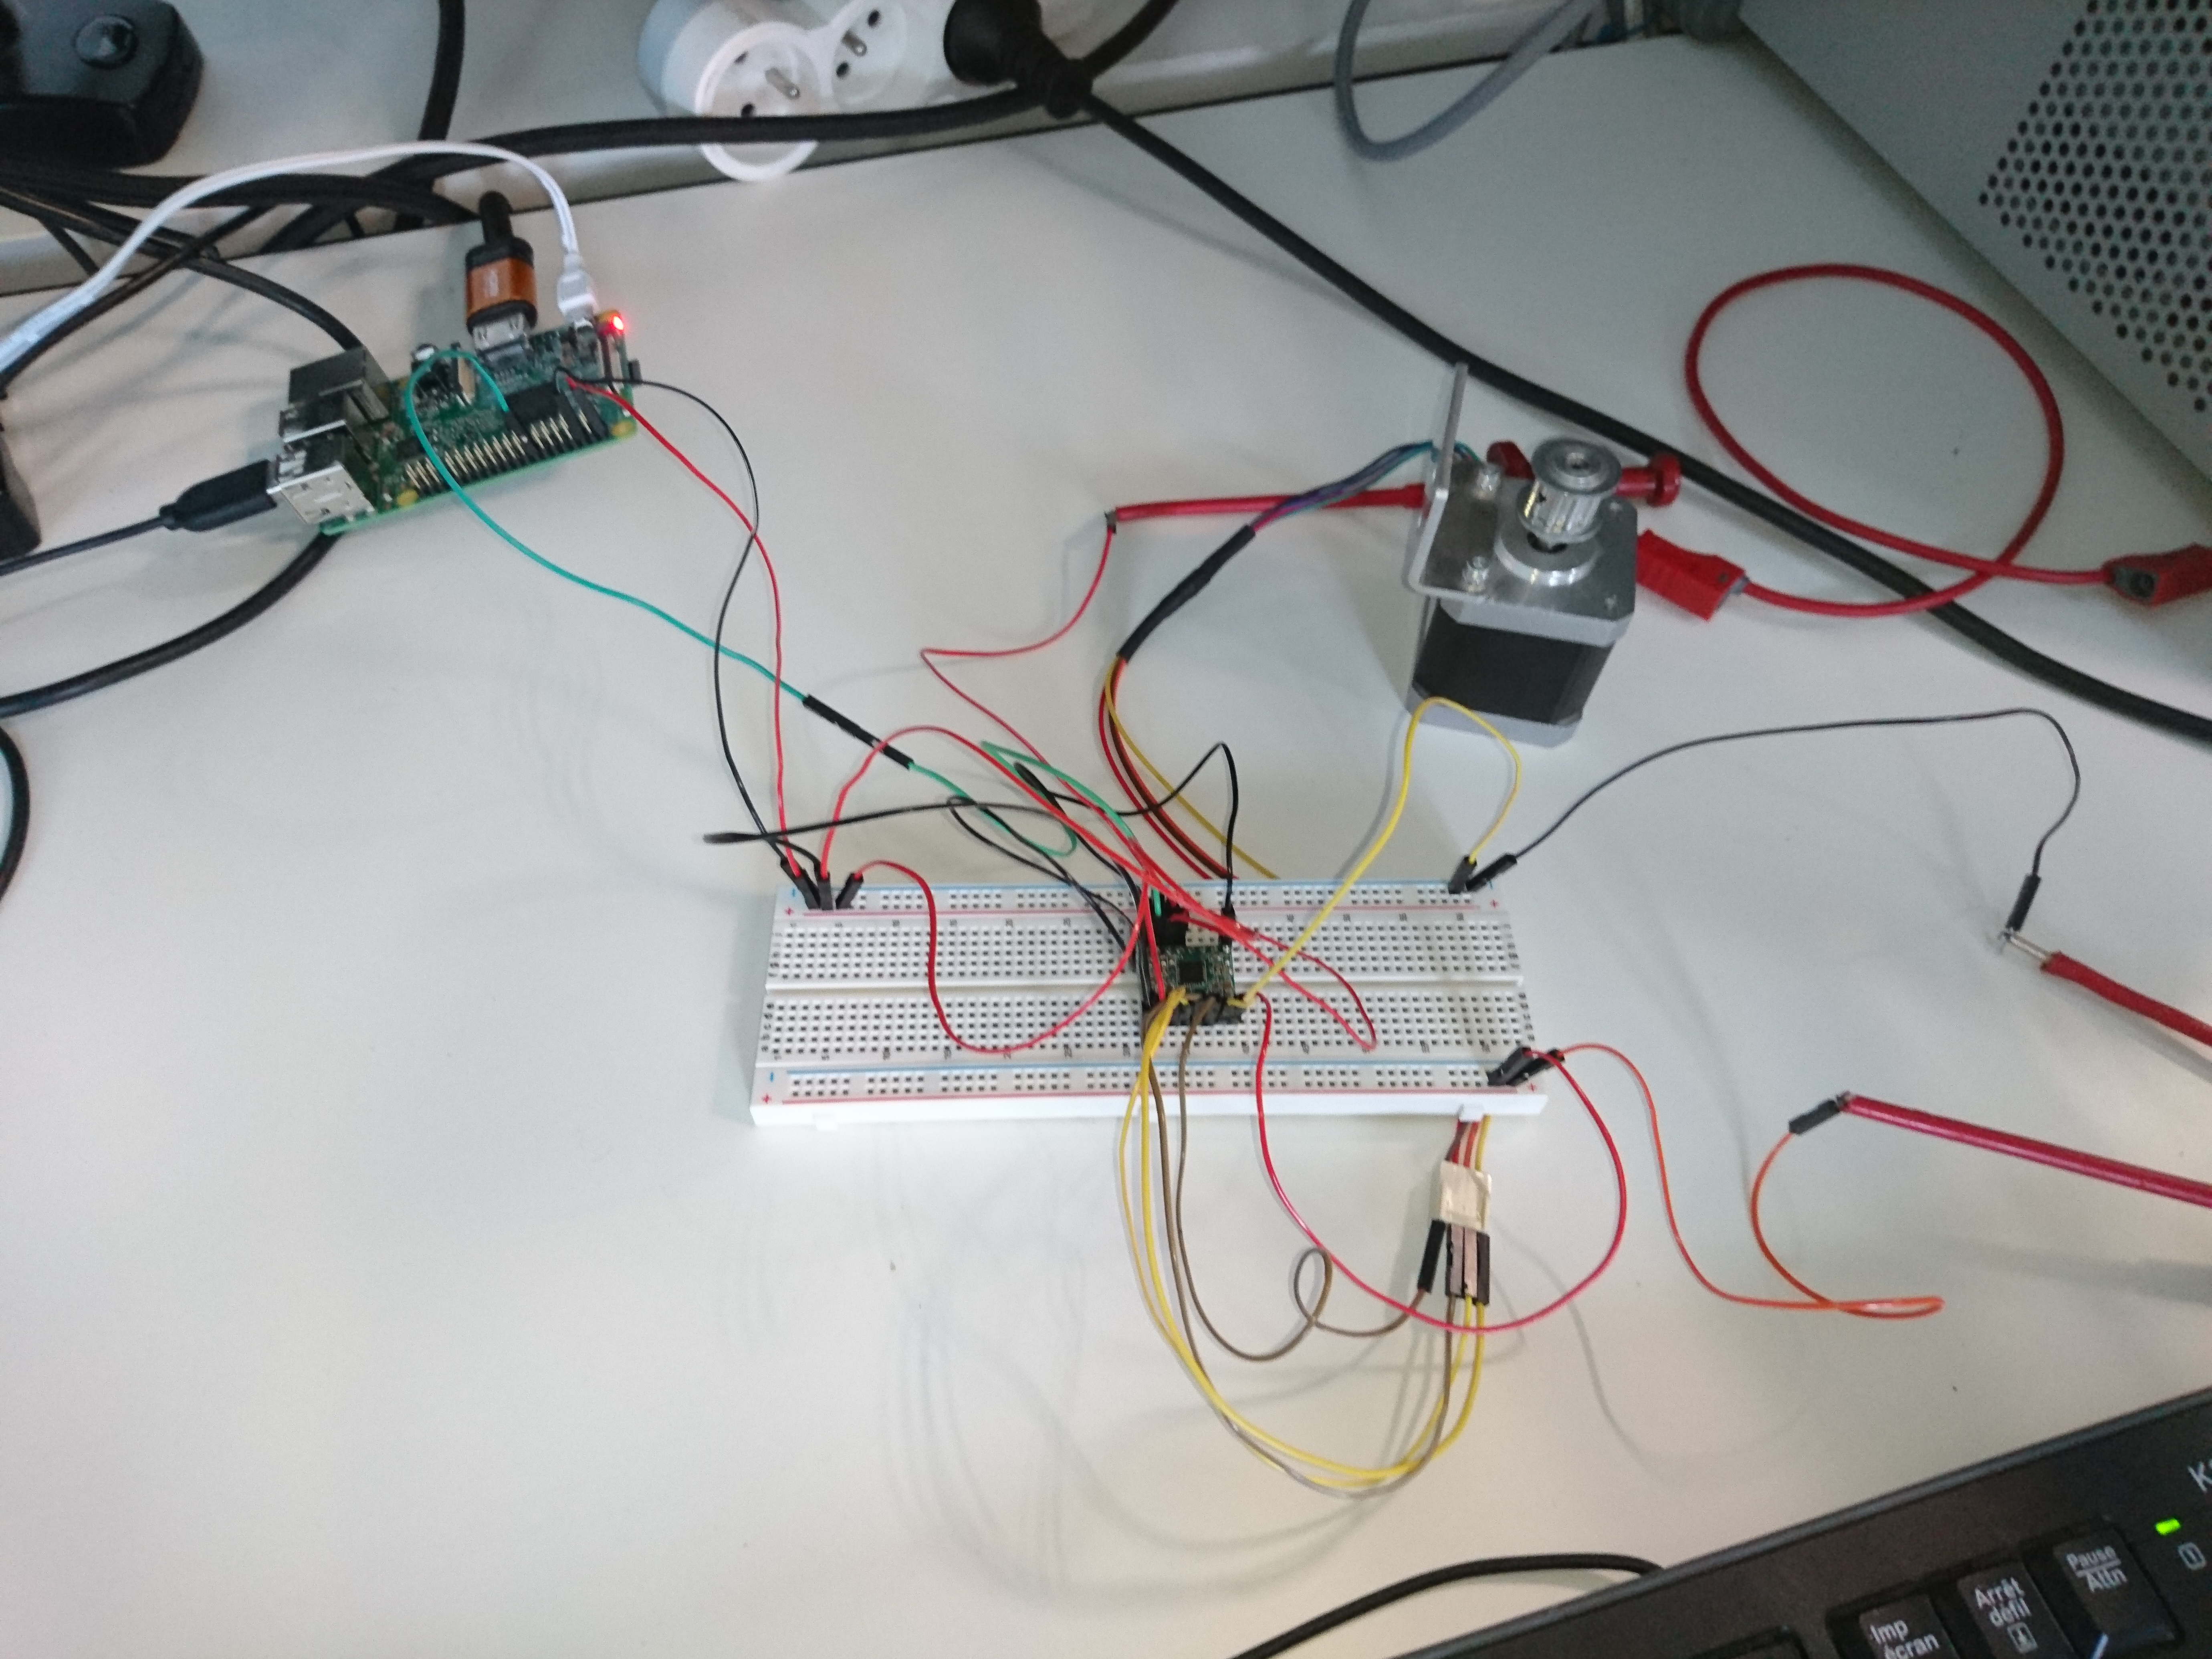
\includegraphics[width=0.9\linewidth]{\figures/photo_test_motor.jpg}
    \decoRule
    \caption[
    Photo du banc de test]{
	Photo du banc de test}
    \label{fig:Photo du banc de test}
    \end{figure}

\vspace{1cm}

J'ai pu valider les fonctionnalités développées, cependant la vitesse max atteinte par le moteur contrôlé par le driver est inférieure à celle que l'on peut atteindre en contrôlant le moteur avec un générateur basse fréquence. Voici le résultat de la commande envoyée par la Raspberry Pi par la pin Step au contrôleur moteur pour faire avancer à chaque front montant le moteur de 1 pas.

\begin{figure}[H]
    \centering
    \includegraphics[width=0.5\linewidth]{\figures/osc_motor.png}
    \decoRule
    \caption[
    Mesure à l'oscilloscope de la commande moteur générée]{
	Mesure à l'oscilloscope de la commande moteur générée}
    \label{fig:Mesure à l'oscilloscope de la commande moteur générée}
    \end{figure}

\vspace{1cm}

Après avoir étudié les résultats avec d'autres professeurs, j'ai conclu que la période minimale que je puisse atteindre soit de $20ms$ est normal. Cette limitation est due au fait que mon driver n'a pas la priorité des ressources dans le Linux. Et que le Linux a un cycle lecture/écriture des entrées/sorties limité. Pour améliorer cela il faudrait passer sur un Linux temps réel.


